% Chapter 5

\chapter{Interface Design} % Main chapter title

\label{Chapter6} % For referencing the chapter elsewhere, use \ref{Chapter1} 

\lhead{Chapter 6. \emph{Interface Design}} % This is for the header on each page - perhaps a shortened title

%----------------------------------------------------------------------------------------
This section provides detailed illustration of the non-interactive and
interactive dynamic energy map implementation and design
choices. After a general overview explaining possible approaches to
add the time dimension in an energy map, the non-interactive energy
map (map animation) approach was presented. For the non-interactive
animation, we briefly discussed the advantages and disadvantages
between different symbol or color representation on the effectiveness
of information convey.

Then a detailed explanation of the dynamic energy map interface is
presented. In this section, we first explained the layout and
functions of each components of the interace and how each component is
designed based on literature studies of dynamic map design. Then we
demonstrated how the dynamic energy map could help to achieve the two
goal functions: 1) identify energy recovery opportunities 2) help
design and sizing of a district energy system

\section{Overview}

Dorling and Openshaw pointed out that dynamic map provides new
potential and possibilities for data analysis but also poses a great
challenge as a result of the less developed theory in space-time
pattern detection and measurement~\cite{Dorling1992}. In order to
better conduct a space-time visualization of the space-time energy
demand information in the dynamic energy map, we based the dynamic
energy map implementation on some literature studies on space-time map
visualization.

Brownrigg mentioned several methods of representing time on a map: 1)
a graph or chart that represents a function over time or a time line
for displaying chronological events 2) sequence of snapshots displayed
over time (animated map) 3) small-multiples of snapshots of changing
states ~\cite{Brownrigg2005}.

Based on the classification above, we applied method 1) and 2) in time
representation for the dynamic energy map project. The dynamic plot of
temporal time series is using method 1) to anchor the quantitative
information. The sequential map image display is using method 2). We
did not used the small multiple method (method 3)). The choice is
based on the following points mentioned by Brownrigg: 1) the number of
snapshots in one display is limited and the finer the detail per
snapshot, the less snapshots one can contain in one display. Since the
3D representation is chosen as one of the major map display methods
(2D map is also available), the level of details per image is
relatively high. This will result in a very small number of multiples
per display~\cite{Brownrigg2005} 2) the subtle changes are easier to
be noticed in the form of animation than with small-multiples
~\cite{Brownrigg2005}. Both drawbacks of small-multiple method will
impair the ability of conveying the rapid temporal changes of
community energy behavior, hence is not suitable for the current
project.

\section{(Non-interactive) Map Animation} \label{anime} 

Map animation was introduced to cartography in
1930s~\cite{Harrower2008}. Its major application of include: 1)
demonstrating the dynamic process of geographic events (weather maps
in weather forecasting is such an example) 2) assisting pattern
recognition and knowledge development for scientific researches. The
study by Dorling and Openshaw is an example of application 2), where
they discovered new leukaemia hotspots through animated
maps~\cite{Dorling1992}.  Animated maps are proven to be more powerful
in conveying the spatial-temporal pattern than static
maps~\cite{McEachern1998}.

The authors used a continuous color encoding method in the creation of
non-interactive animation of a univariate gas heating energy demand
map. A red to blue color ramp is used in the map display. Each color
within this red-to-blue color scheme is represented as a real number
between 0 and 1 with 0 representing pure red and 1 representing pure
blue. A log-scaling was performed to the energy data to ``flatten''
the distribution. Then the normalized distance between the current
demand and the maximum demand is calculated with \eref{eq:log}. A
snapshot of the animation is shown in \fref{fig:anime0002}. The
animation can be viewed and downloaded
\href{http://www.armechxyj.com/energy-mapping.html#colorAnime}{through
  this link}

\begin{figure}[h!]
  \centering
  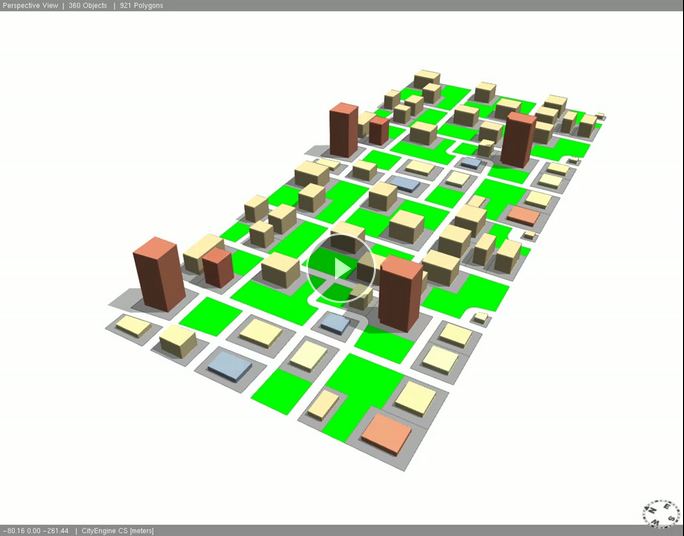
\includegraphics[width=0.5\linewidth]{img0002.png}
  \caption[Animated Map with Continues Encoding]{Animated Map with
    Continues Encoding}
  \label{fig:anime0002}
\end{figure}

In the dynamic energy map interface design, we applied a discrete
color encoding with a seven-class bivariate choropleth representation
because it can create a legend that can depict more specific quantity
information. An animation with this discrete color scheme is also
created and can be viewed and downloaded
\href{http://www.armechxyj.com/energy-mapping.html#redblueAnime3d}{through
  this link}. Although the initial conditions of the map instances
using the continuous and discrete encoding method are different, we
ovserved that the continuous color encoding method seems to be better
in demonstrating the general pattern of energy changing
behavior. Further evaluations are needed to compare these two
approaches and justify the design choice of a discrete or continuous
color scheme.

\begin{figure}[h!]
  \centering
  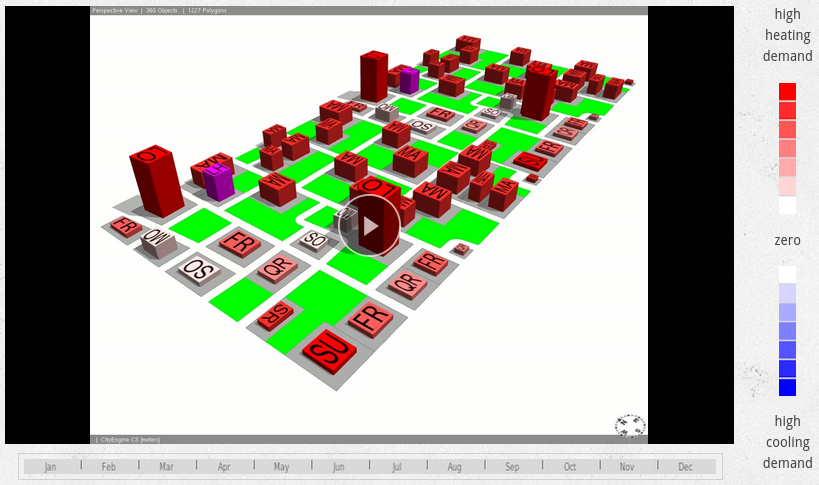
\includegraphics[width=0.5\linewidth]{forPublic.png}
  \caption[Animated Map with Discrete Encoding]{Animated Map with
    Discrete Encoding}
  \label{fig:anime0002}
\end{figure}

Dong et al.\ assessed the effectiveness of symbol design and frame
rate on the effectiveness of dynamic map display with two performance
measurements: deviation and response time. They identified the optimal
class numbers is 15 for graduated size symbol and is 10 for graduated
color symbol on a 1024x768 display. The optimal frame rate identified
in the study is 3 for color symbol maps and 6 for size symbol
maps. They also suggest to reduce class number and frame rate if the
display size is smaller than
1024x768~\cite{doi:10.1559/1523040639298}. 

The non-interactive animated map display has size of
$1213 \times 950$, a little larger than that of the suggested display,
we thus chose the frame rate to be 4 per second.

\section{Interactive Dynamic Map Interface}
\subsection{General Layout}
The general layout of the dynamic map interface is displayed in
\fref{fig:interfaceLayout}. It contains the following major sections :
\begin{figure}[h!]
  \centering
  \begin{subfigure}{0.7\textwidth}
  \centering
  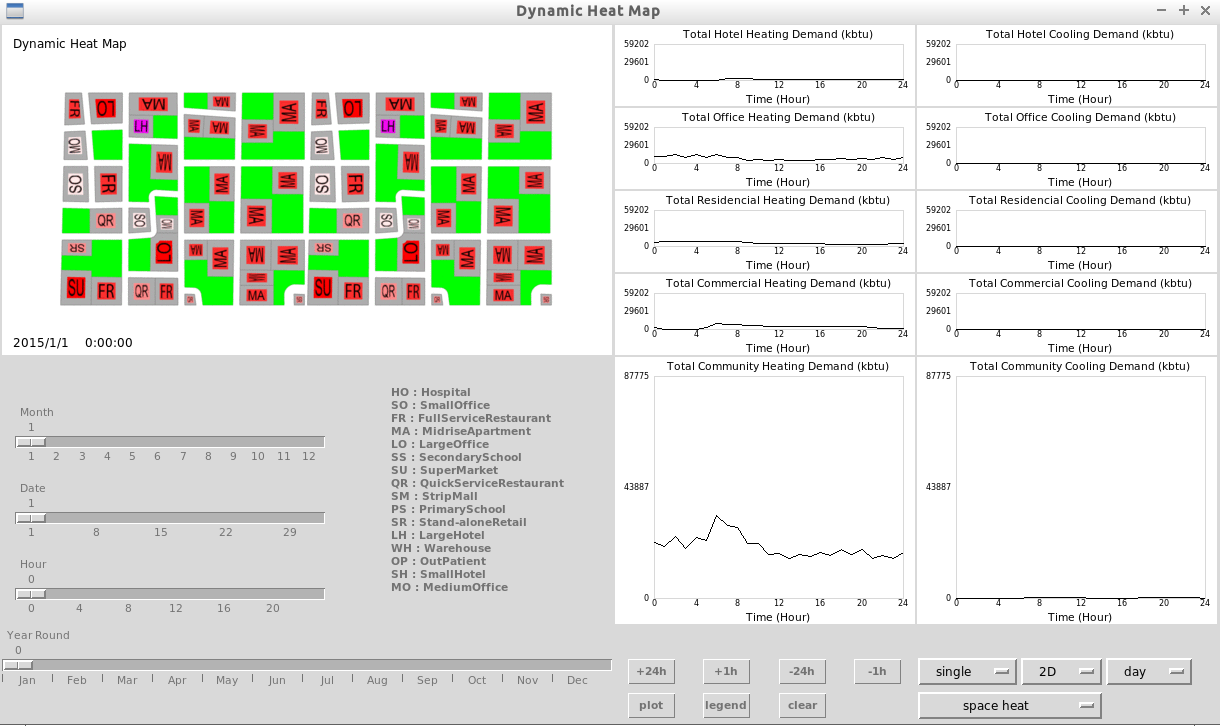
\includegraphics[width=\linewidth]{interface08}
  \caption[Dynamic Energy Map Interface Snapshot]{A snapshot of the dynamic energy map interface}
  \label{fig:interface08}
\end{subfigure}
~
\begin{subfigure}{0.7\textwidth}
  \centering
  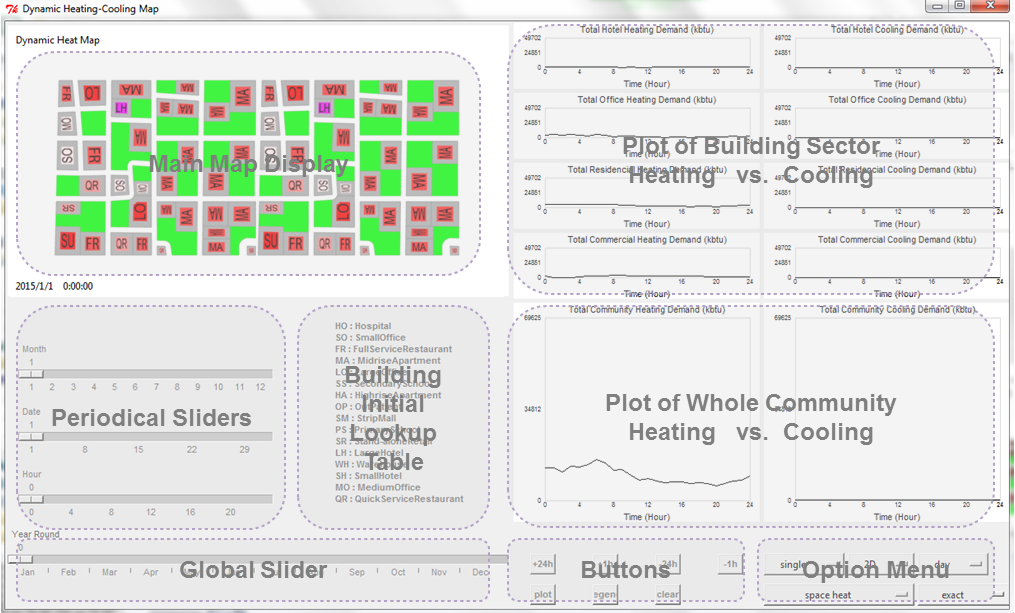
\includegraphics[width=\linewidth]{layout08.png}
  \caption[Dynamic Energy Map Interface Layout]{Dynamic Map Interface Layout}
  \label{fig:layout08}
\end{subfigure}
\caption{Dynamic Map Interface Layout}
\label{fig:interfaceLayout}
\end{figure}

\begin{itemize}
\item A main map display on the upper left that shows the 2D or 3D
  version of the dynamic energy map with energy data encoded as the
  color of buildings. 

\item Four sliders that controls the linear and periodical navigation
  of the map image display and data plot.

\item A ``Building Initial Look-up Table'' in the center bottom that
  explains the building type initials on the main map display window.
\item A series of energy demand plots for four major building sectors
  (top right) and the whole community (lower right).  
\item A series of buttons and option menus on the lower right. 

  The top row of the buttons performs forward (+) or backward (-) time
  navigation with time step of 24h or 1h. The bottom row of the
  buttons contains a ``plot'' button that plots the energy profile
  graphs of the 16 benchmark buildings (if ``single'' is chosen for
  option menu'') or the plot of the aggregated community (if
  ``community'' or ``group'' is chosen), a ``legend'' button that
  shows the current legend, and a ``clear'' button that clears the
  selection in the 2D mode (\fref{fig:optionMenu}).
  
  \begin{figure}[h!]
    \centering
    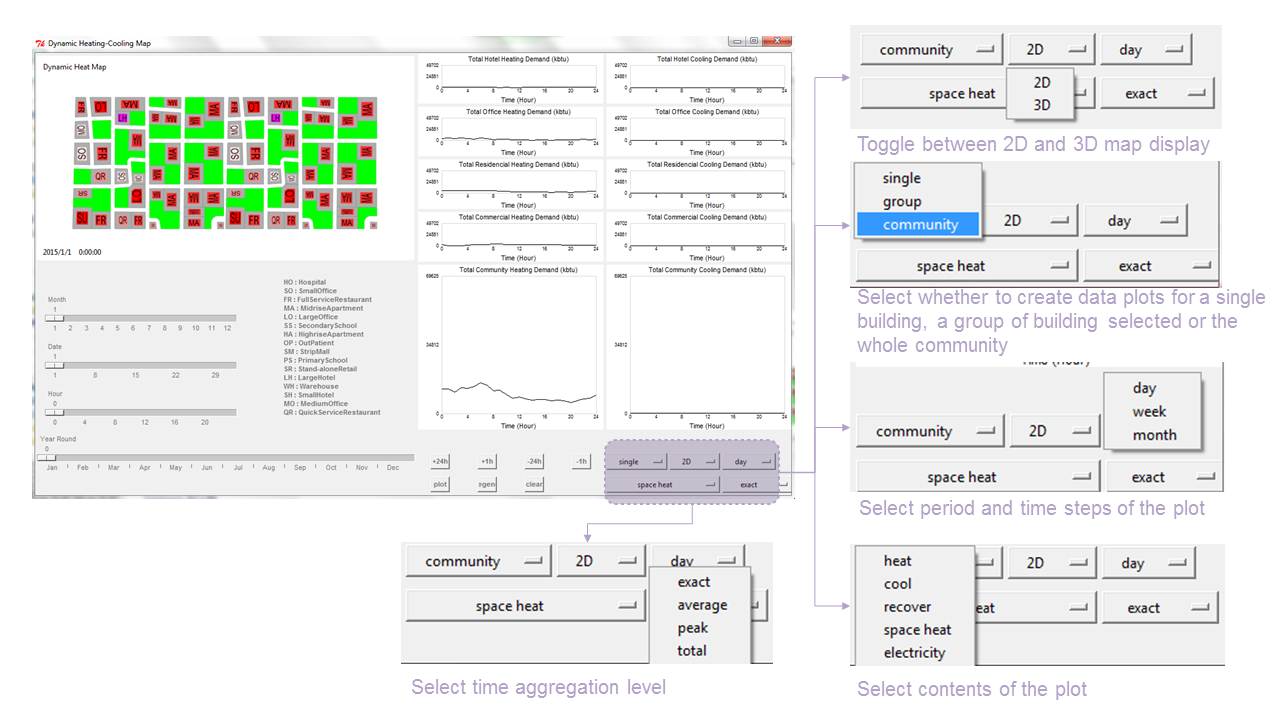
\includegraphics[width=0.7\linewidth]{optionMenu.png}
    \caption[Option Menu]{The option menu contains a 2D/3D toggle,
      several plotting options determining the plotting topic (space
      heating, cooling, energy recovery potential, heating and
      electricity), the plotting time step and duration (month, week,
      day) and the buildings involved in the plot (single, group, community)}
    \label{fig:optionMenu}
  \end{figure}

\end{itemize}

The following sections will provide more detailed explanation of the
interface.

\subsection {Main Display Window} \label{2d3d} 

As is mentioned in ~\cite{Brownrigg2005}, the choice of 2D
representation vs. 3D representation is one of the debating decisions
in the world of cartographic data
visualization~\cite{Brownrigg2005}. 2D maps are 1) easier to navigate
through and 2) easier to perform selection and manipulation. Another
important advantage of 2D map is that it has better theory
support~\cite{Resch2014} while the principles and variables of 3D or
4D maps (space-time map) are not thoroughly
investigated~\cite{Resch2014}. This situation makes the design of 3D
maps more difficult. However 2D maps ``drastically simplify reality
and thus do not give credit to the highly complex capabilities of
human spatial cognition''~\cite{Resch2014}. Regarding this, 3D map is
rich in geometry representation and can provide realistic scenes. This
feature can both be an advantage or disadvantage based on the actual
map usage. According to Tufte's data-ink ratio theory, the extra
non-crucial richness of information should be eliminated to make the
most important information stand out~\cite{Tufte83}.

For the current dynamic energy map interface, both 2D and 3D
representations are provided for the users to select.  The main map
display window on the top left is used for displaying the 2D / 3D
dynamic map of the conceptual model. The lower left of the main map
display window displays the current time for the image and data
plots. By selecting the 2D / 3D option in the option menu on the lower
right, the user can choose between 2D and 3D display. The 3D display
provides a more realistic view of the community model. The building
geometry is simplified in the current model in order to emphasize the
color changing between frames without introducing distraction from
complicated building geometry. Additional building details or features
could be added to make the display more realistic. In the 2D display,
user can click on a single building or select a group of buildings to
display their energy profile plots or the aggregated energy profile
plots (\fref{fig:2d3dSelect}).

\begin{figure}[h!]
  \centering
  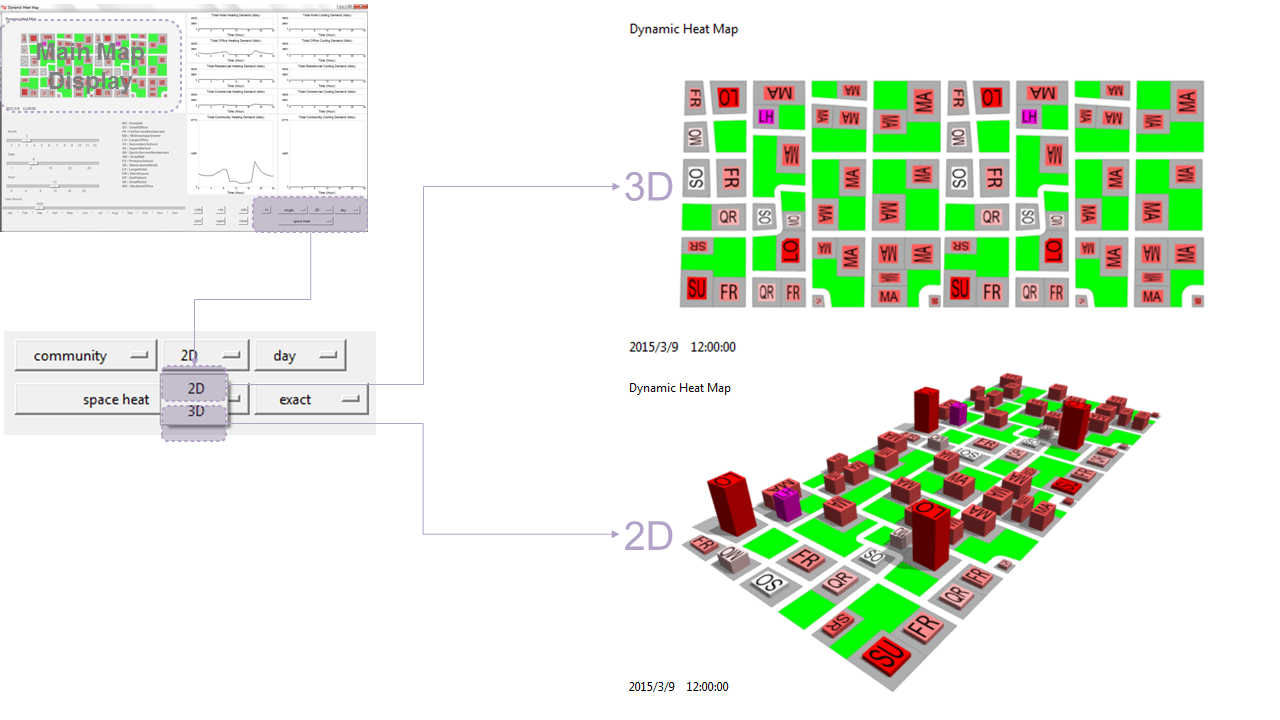
\includegraphics[width=0.7\linewidth]{2d3dSelect.png}
  \caption[Map Display of 2D and 3D]{The current interface provides
    the choices of viewing 2D and 3D map display by toggling the 2D/3D
    option menu}
  \label{fig:2d3dSelect}
\end{figure}

\subsection{Bivariate Map Legend} \label{bivariate}

\subsubsection{Symbol Chosen}
Our major intention for choosing the 3D energy dynamic map display is
to use it to provide a more realistic urban environment context.  In
the Dutch Heat map by Dobbelsteen et al.\ , the quantity of energy
demand of each building or region is represented by extruding the
building or region by a corresponding height encoding its energy
demand or supply ~\cite{Dobbelsteen2013}. This approach provides an
easy way of aggregating energy demand and supply by adding up geometry
height, but this approach is not suitable for our map design because
it creates shape distortion and will impair our goal of providing a
realistic urban environment vision.

In order to represent space heating demand and cooling demand on the
same map, a common map design problem is encountered in the current
project: bivariate map design problem. Elmer presented eight possible
types of representation for bivariate maps (\fref{fig:bivariateExp}):
``shaded cartographer, rectangle map, bar chart, value by alpha,
choropleth with graduated symbol, bivariate choropleth, spoke glyph
and shaded texture''~\cite{Elmer2012}. In order to incorporate the
bivariate map symbols to the current 3D model without introducing too
much shape distortion, we did not choose the representation with
dimensional changes. The only choices are the ones that only involves
color or texture, i.e. ``bivariate choropleth, value by alpha and
shaded texture'' (\fref{fig:bivariateExp}). Among these three choices,
bivariate choropleth representation has the highest accuracy
rate~\cite{Elmer2012}, hence we choose bivariate choropleth as the
representation of the current map interface design.

\begin{figure}[h!]
  \centering
  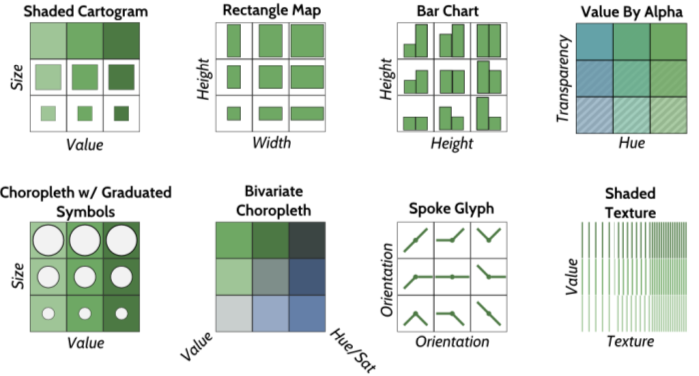
\includegraphics[width=0.7\linewidth]{bivariateExp.png}
  \caption[Bivariate Map Symbol Tested]{The eight bivariate map
    display approaches tested in Elmer's~\cite{Elmer2012} study}
  \label{fig:bivariateExp}
\end{figure}

\begin{figure}[h!]
  \centering
  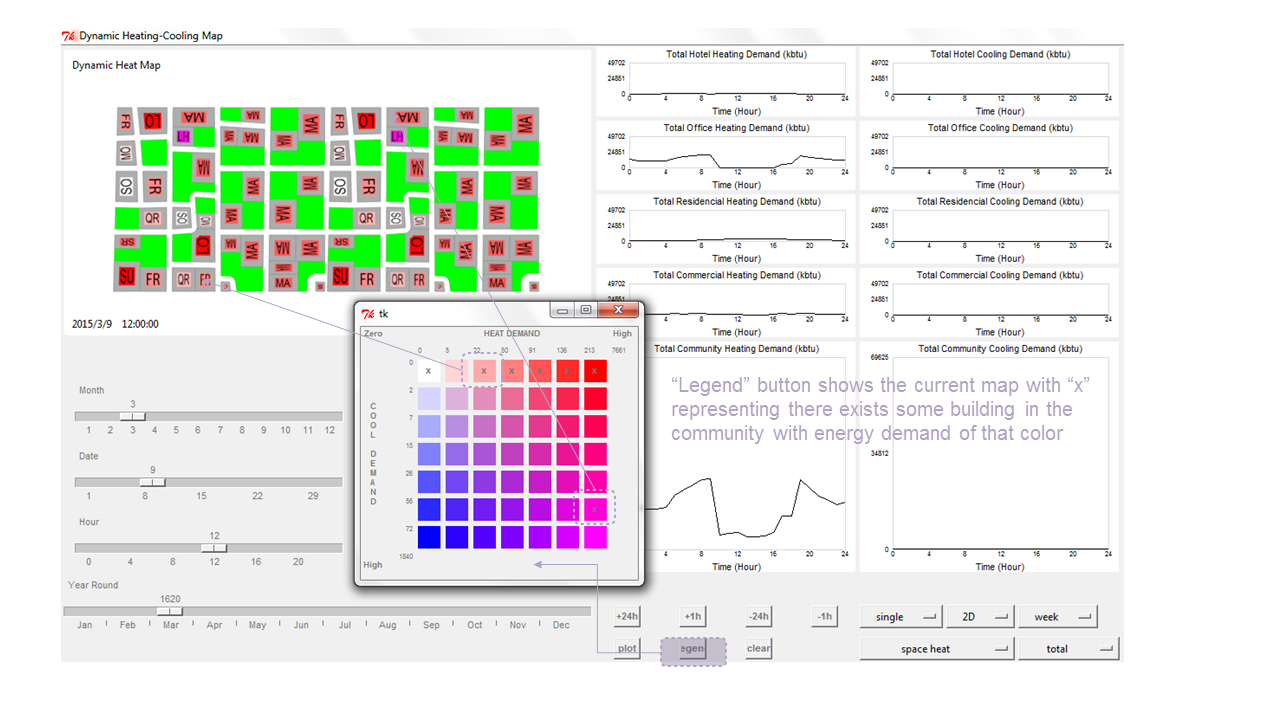
\includegraphics[width=0.7\linewidth]{legend.png}
  \caption[Bivariate Map Legend]{The seven-class-bivariate choropleth
    legend is used in the dynamic energy map interface design with red
    representing high space heating demand, blue representing high
    space cooling demand. ``x'' in the legend corresponds to colors
    appear in the current map display window}
  \label{fig:legend}
\end{figure}

In the current interface design, users can click on the ``Legend''
button and a legend used for encoding the 2D and 3D map will be
displayed. To assist legend reading and color comparison between the
map and the legend, tick marks of ``x'' are added to the legend to
indicate the color appeared in the map \fref{fig:legend}.

\subsubsection{Data Classification}\label{dataClassification}
A function from energy data value to its color representation should
be decided in order to visualize energy data in a map display. A
common approach is to create a series of graduated color or symbol and
classify the data into a few groups and assign each group one color or
symbol in the series of symbols. In order to write the data
classification routine for the demonstration of dynamic energy map in
the current study, the authors conducted a brief survey of the
commonly used GIS software for commonly applied data classification
methods. The software surveyed in the study include:
ArcGIS~\cite{GIS_Jenks2014}, GRASS GIS~\cite{GRASSGIS2008},
gvGIS~\cite{gvGIS2011}, and QGIS. The data classification method
adopted by the surveyed software in creating a thematic map include:
1) equal interval, 2) quantile 3) Jenks 4) Standard Deviation 5)
pretty breaks and 6) manual interval (use context specific break point
values). The common data classification method shared by all surveyed
instances are ``Equal Interval'', ``Quantile'' and ``User
Defined''. Therefore we chose to implement the ``Equal Interval'' and
``Quantile'' method in the current project.

\begin{table}[h!]
  \centering
  \begin{tabular}{r|c c c c c c}
    \hline
           & Equal Interval & Quantile & Jenks & Pretty Breaks & StDev & User Defined\\
    \hline
    ArcGIS &      o        &    o     &  o    & x &  o  &   o  \\
 GRASS GIS &      o        &    o     &  x    & x &  o  &   o  \\
     GVSIG &      o        &    o     &  o    & x &  x  &   o  \\
      QGIS &      o        &    o     &  o    & o &  o  &   o  \\
    \hline
  \end{tabular}
  \caption{Data Classification Method (o: yes, x: no)}
  \label{tab:classify}
\end{table}

From the distribution of energy data point in \cref{Chapter4}, we
observed a severe right skew of the energy data distribution of single
buildings and the community, if using the ``Equal Interval'' method,
the display will lack variation between different frames because the
majority of data points will be concentrated in low-energy demand
end. For ``User Defined'' breakpoints, further study or survey will be
necessary to decide the set of robust breakpoints based on specific
building energy context. The ``Quantile'' method is thus chosen as the
data classification method for the demonstration of the functions of
the dynamic energy map interface.

\subsection{Time Sliders and Navigation Buttons}
The lower left section contains a series of sliders for controlling
interactive navigation of the image sequence and corresponding data
plot. 

Harrower and Fabrikant classify time into two types: linear and
cyclic~\cite{Harrower2008}. The former represents the periodical
changes and the latter represents the linear changes of spatial
temporal variables. Upon this consideration, the design of the current
interface include both an overall time navigation utility and time
navigation utilities that facilitate jumps with time steps
corresponding to the natural period of energy data, such as month, day
and hour. This design choice is anticipated to facilitate the
representation of both linear changes and periodical changes of energy
usage in the community.

There are three shorter ``periodical'' sliders on the lower left of
the interface. One unit of position change in the ``month'' slider
results in a forward or backward jump of one month in time. The total
number of positions in the ``month'' slider equals to the number of
months in a year (which is the next level of time unit regarding
month).  The jump step for ``date'' slider is one day and the number
of positions in the ``date'' slider is the number of days per
month. Similarly for the ``hour'' slider, the jump step is one hour
and the number of positions in ``hour'' slider is the number of hours
per day. Suppose the current time in display is 2015/1/1 12:00:00, by
moving the month slider, viewers can see the energy demand in the from
of map image and data plot for 2015/2/1 12:00:00, 2015/3/1 12:00:00,
$\dots$, 2015/12/1 12:00:00. Similarly, if views pull the ``date''
slider, they can compare the different energy demand of this hour
(12:00:00) throughout the whole month. For hour slider, viewers can
compare the energy demand between different hours of a day.

There is a longer ``linear slider'' on the bottom left of the
interface. It has a time step of an hour and a navigation range of a
year (8760 hours). It allows users to globally navigate through all
8760 hours of the year.

There are four buttons (+24h, +1h, -24h, -1h) on the bottom right of
the interface. They provide a micro level adjustment of time.

\subsection{Data Plot}
\subsubsection{Methods to Show Plot}
There are three ways to view energy data plots in the dynamic energy
map interface:
\begin{enumerate}[1)]
\item By viewing the right hand side of the interface.

  The dynamic data plot are directly shown on the right of the
  interface. They depict the energy demand of the four major building
  sectors (Hotel, Office, Residential and Commercial buildings) and
  the community.

  Space heating and cooling energy demand is displayed in
  \fref{fig:interfaceLayout}. The interface can also display the
  electricity and heating demand for the CHP plant sizing
  application. These plots starts from the current time showing on the
  time sliders with a fixed plotting range of 24h.

\item By clicking on the ``plot'' button on the lower right of the
  interface.

  If the ``single'' option in the option menu is chosen before one
  clicks the ``plot'' button, a data plot will be created for each
  building type (\fref{fig:singlePlot}). If the ``community'' option
  in the option menu is chosen before one clicks the ``plot'', a data
  plot for the community will be created (\fref{fig:communityPlot}).

  \begin{figure}[h!]
    \centering
    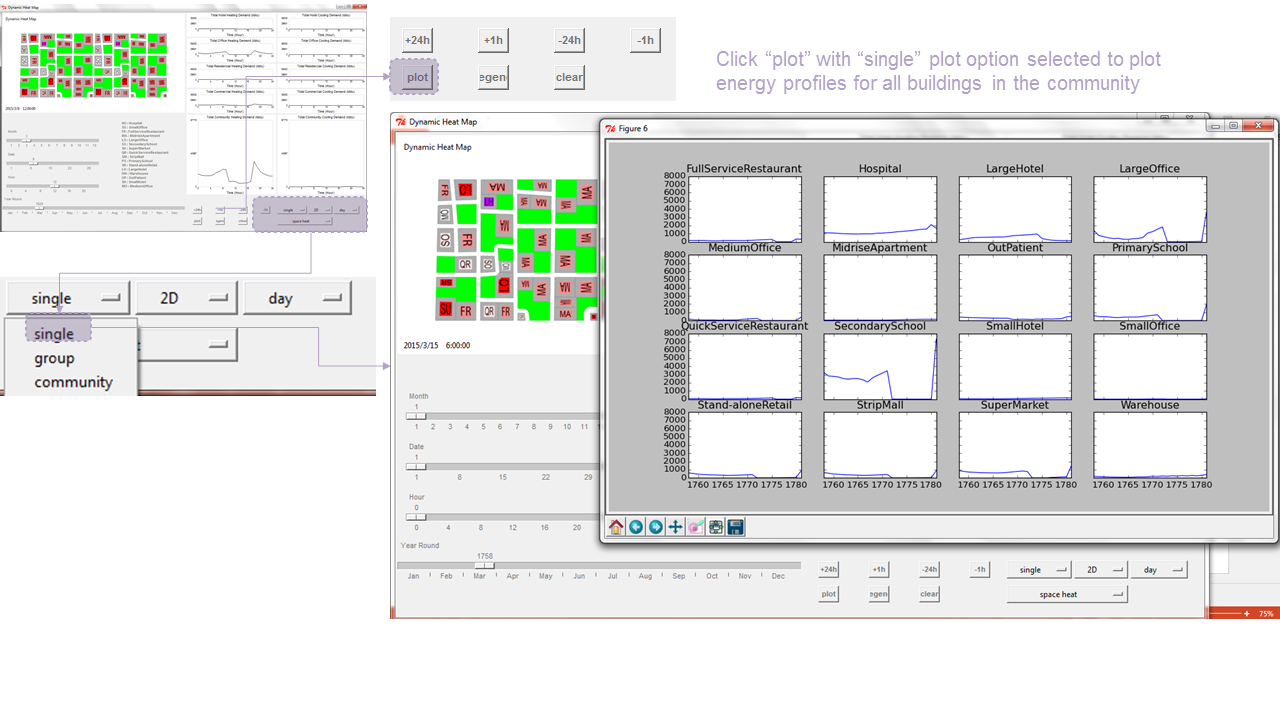
\includegraphics[width=0.9\linewidth]{singlePlot.png}
    \caption[Single Plots of 16 Building Types]{The plot shows the
      space heating energy demand plot of each of the 16 benchmark
      buildings}
    \label{fig:singlePlot}
  \end{figure}

  \begin{figure}[h!]
    \centering
    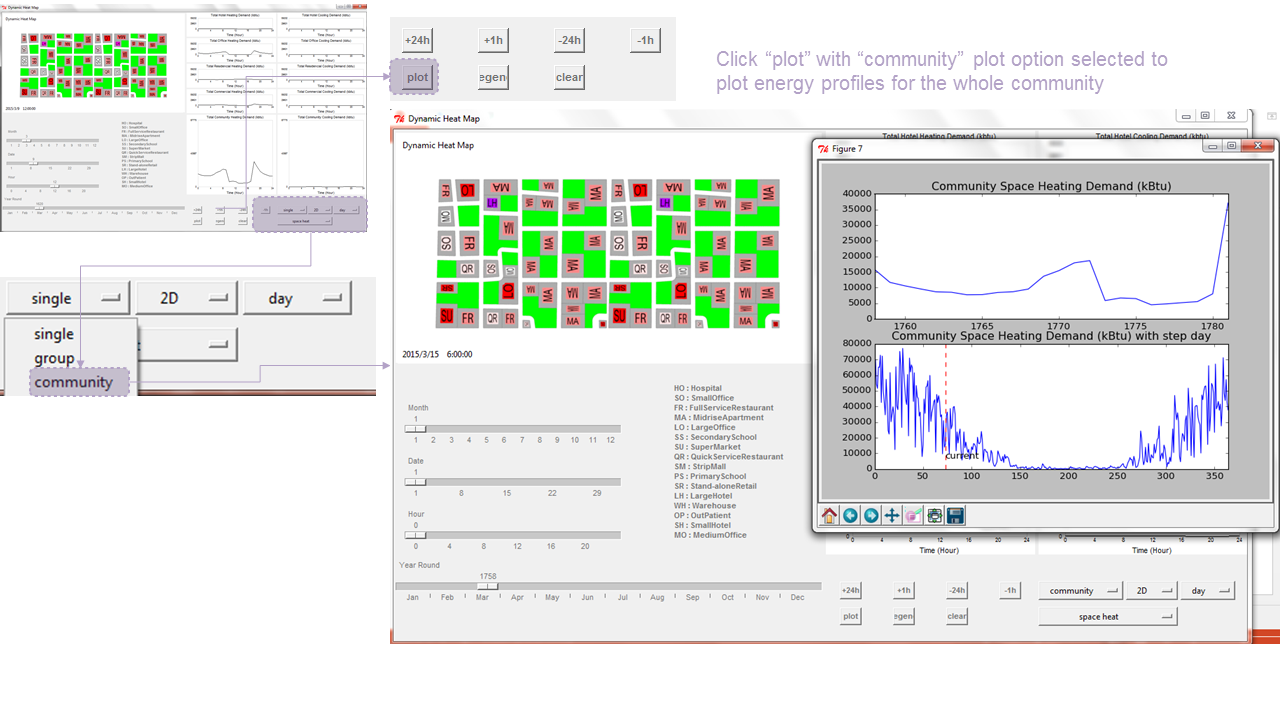
\includegraphics[width=0.9\linewidth]{communityPlot.png}
    \caption[Community Plot]{The plot shows the aggregated space
      heating energy demand for the whole community}
    \label{fig:communityPlot}
  \end{figure}

\item By clicking on the building foot print in the 2D map display.

  A building is ``selected'' if the user clicks on its foot
  print. Each new click of a building foot print will add a new copy
  of that building to the selection set. The selection set can be
  cleared by pressing the ``clear'' button. If ``single'' option is
  chosen in the option menu before clicking on a building's foot
  print, a data plot will be created for the building the viewer just
  clicked on (\fref{fig:clickSingle}). If ``group'' is chosen in the
  option menu, each click of a building's foot print will create a
  data plot for the current selection set (\fref{fig:clickGroup}).
  
  \begin{figure}[h!]
    \centering
    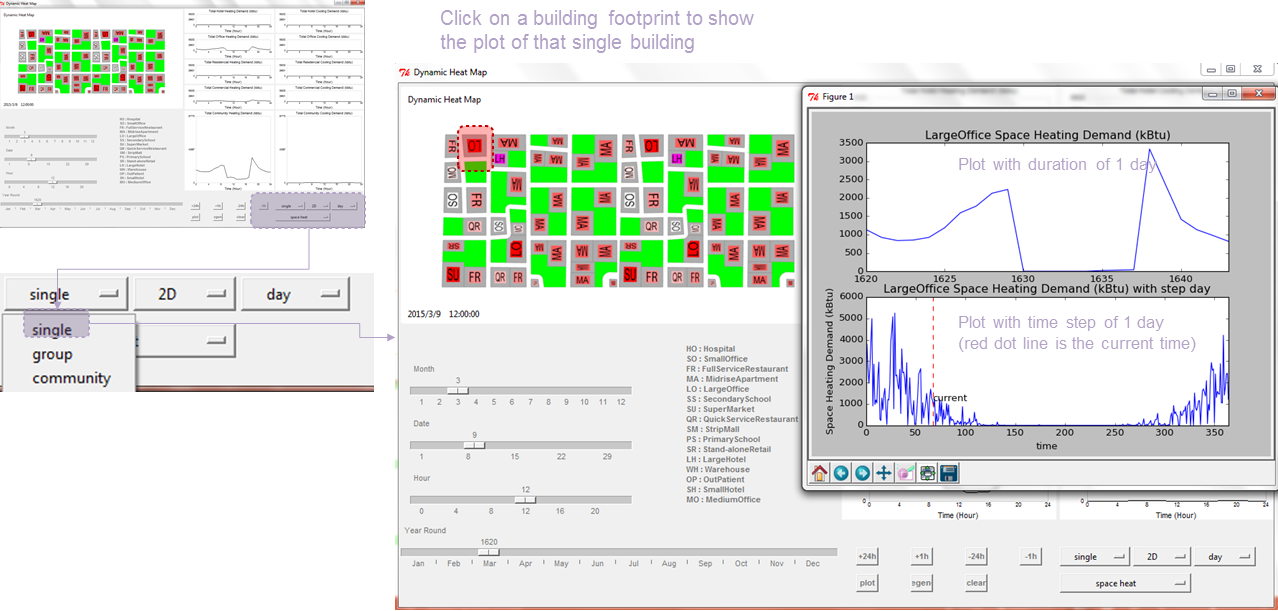
\includegraphics[width=0.9\linewidth]{clickSingle.png}
    \caption[Show Plot for One Building]{Click on a building foot
      print shows the energy plot of this building}
    \label{fig:clickSingle}
  \end{figure}

  \begin{figure}[h!]
    \centering
    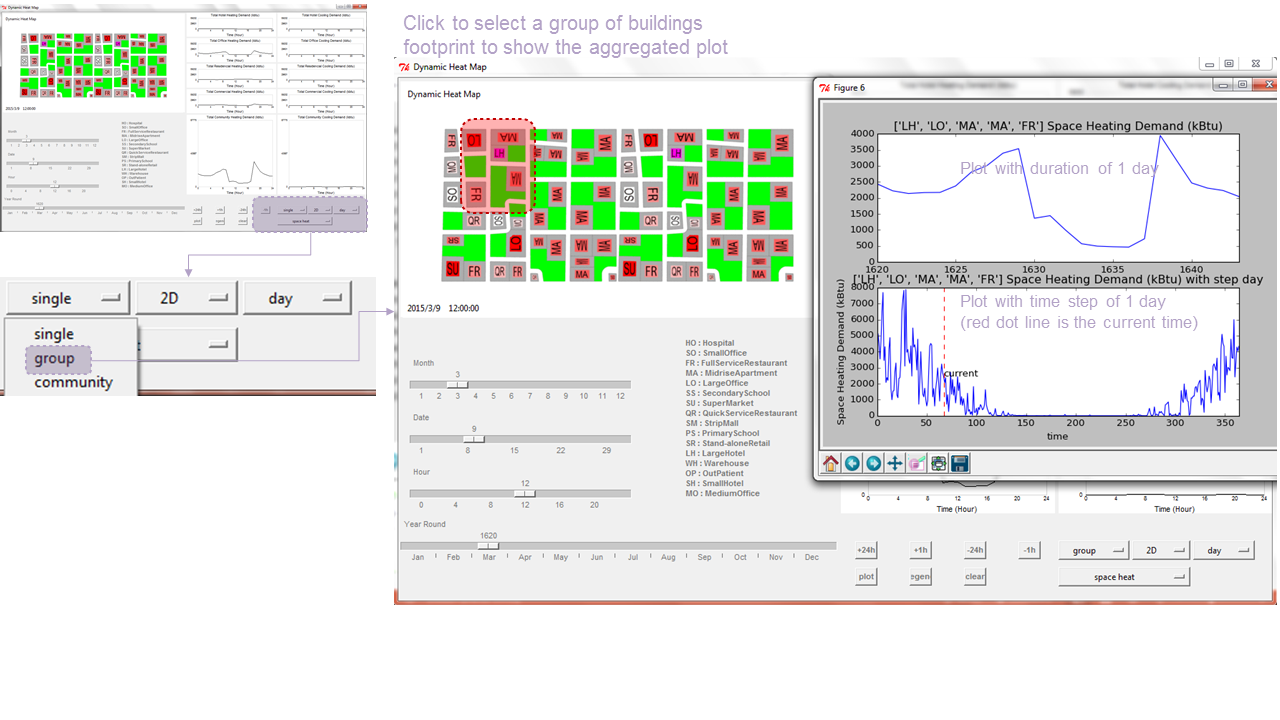
\includegraphics[width=0.9\linewidth]{clickGroup.png}
    \caption[Show Plot for a Group of Buildings]{Click on a building
      foot print shows the energy plot for the selected building group}
    \label{fig:clickGroup}
  \end{figure}

\end{enumerate}

\subsubsection{Providing Temporal Context in Data Plot}

Brownrigg suggested that it is necessity to provide the ``temporal
context'' in a space-time map: ``To comprehend how drastically or
subtly something is changing, how fast or slow, in what direction, in
relative to its environment, etc., demands some knowledge of the
history of the change, an awareness of the objects' properties before
and after the change.''~\cite{Brownrigg2005}.

In the current map image display, the temporal context is created by
providing three ``periodical'' slider bars that allows the user to
jump with time steps of month, day and hour. 

In data plots, the temporal context is created by providing a
``longitude'' and ``latitude'' comparison of energy demand.
``Longitude'' here refers to the comparison of adjacent time spots. It
shows what the states of the direct future or past comparing to the
state of the current time. ``Latitude'' here refers to the comparison
of the current time spot with all similar time instances, for example,
all 12:00:00 energy demand of the year. It shows how the current
instance differ from similar instances.

For the current interface design, the top plot presents a longitude
temporal context of the energy demand of the incoming 24h, week or
month. Corresponding to the duration of time of the top plot (24h or
one week or one month), the bottom plot presents the latitude demand
context of the same hour with a step of one day, one week or one
month. For example, in \fref{fig:dayContext}, the top plot shows the
Space Heating Demand for Large Office from 2015/3/9 12:00:00 to
2015/3/10 11:00:00, with a duration of 24h. The bottom plot shows the
energy demand of the Large Office for all 12:00:00 of the 365 days of
the year (the red dot line indicates the 12:00:00 of around the 70th
day of the year, which is the date of Mar. 9th).

\begin{figure}[h!]
  \centering
  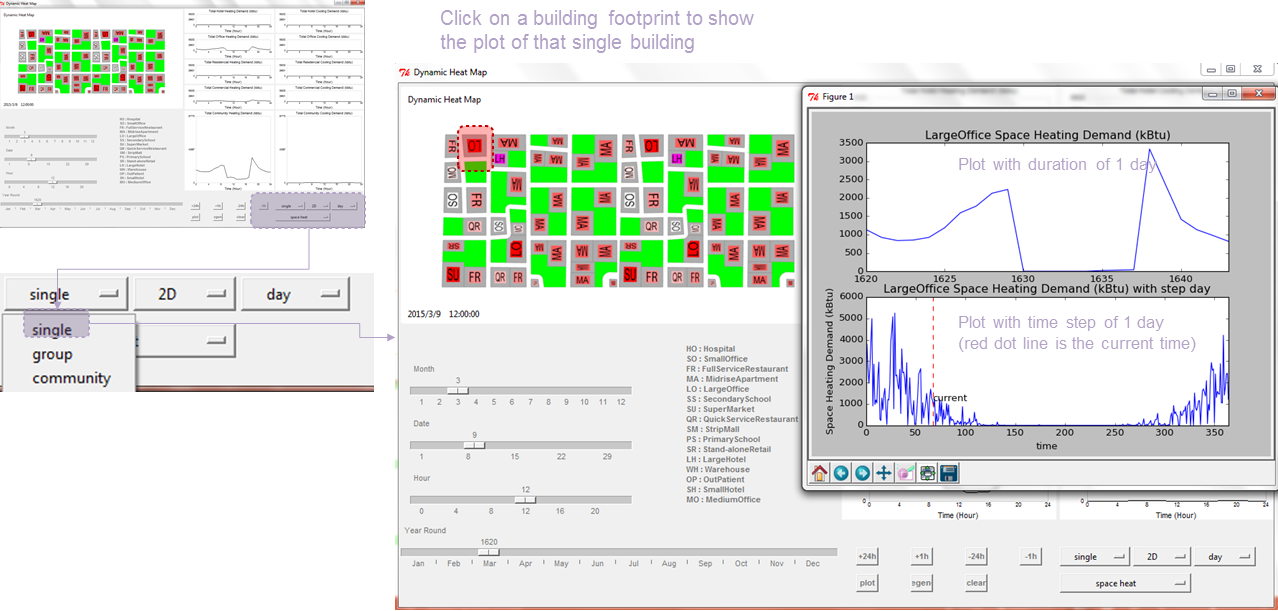
\includegraphics[width=0.9\linewidth]{dayContext.png}
  \caption[Data Plot with Duration / Step of One Day]{The data plot
    presents the longitude and latitude comparison of energy demand,
    the top plot presents a temporal context of the energy demand of
    the next 24h, the bottom plot presents the time context of the
    demand of the same hour throughout the 365 days of the year}
  \label{fig:dayContext}
\end{figure}

\begin{figure}[h!]
  \centering
  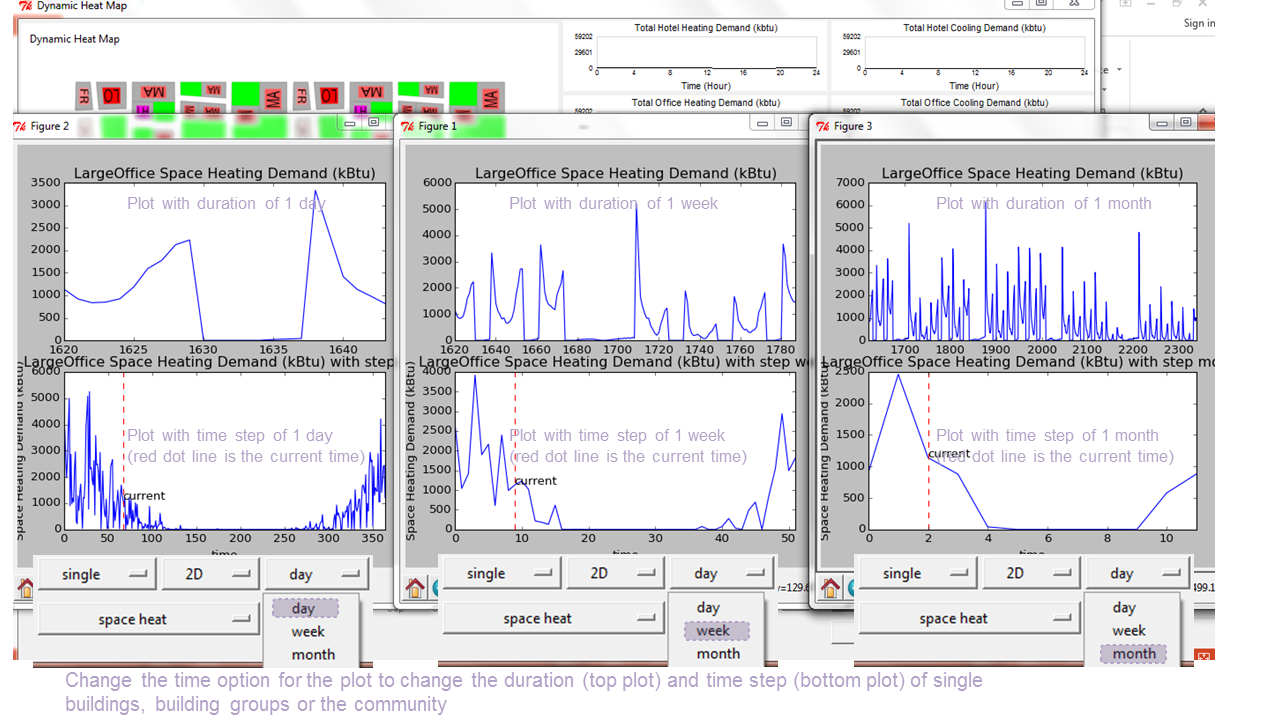
\includegraphics[width=0.9\linewidth]{changeT.png}
  \caption[Data Plot with Different Duration / Step]{By changing
    option in the option menu. User can choose to display a longitude
    latitude comparison with the time unit of day, week or month. The
    top plot shows the energy demand for the next day, week and month
    from left to right; the bottom plot shows the energy demand of
    this hour in the 365 days of year, 52 weeks of a year or the 12
    months of a year from left to right}
  \label{fig:dayContext}
\end{figure}

By providing the temporal context, we would like to provide viewers
with a general understanding of whether the changing of energy demand
behavior is drastic or subtle and whether a drastic change is coming
and whether the current demand is high, low or moderate comparing to
the overall distribution over time and space.

\pagebreak
\section{Use Case Demonstrations}
\subsection{Use Case I: Identification of Energy Recovery Opportunity}
In this section, we present a general approach on how to use the
dynamic energy map interface to identify the energy recovery
opportunities. The process of space cooling will produce reject
heat. As is explained in \sref{sec:inputRecover}, the ammount of
cooling induced reject heat is positively corelated to the cooling
demand. Thus a building with high cooling demand will also has a large
amount of reject heat. The reject heat from this building or group of
buildings could be recovered by itself or be transmitted to other
buildings that has space heating demand so that the total space
heating demand of the group of buildings could be reduced.

With the dynamic energy map, the buildings colored in one of the
colors in the bottom rows of the legend are buildings with high
cooling demand. With the dynamic energy map, one can identify
the potential reject heat suppliers and consumers over time
(\fref{fig:highCooling}).

\begin{figure}[h!]
  \centering
  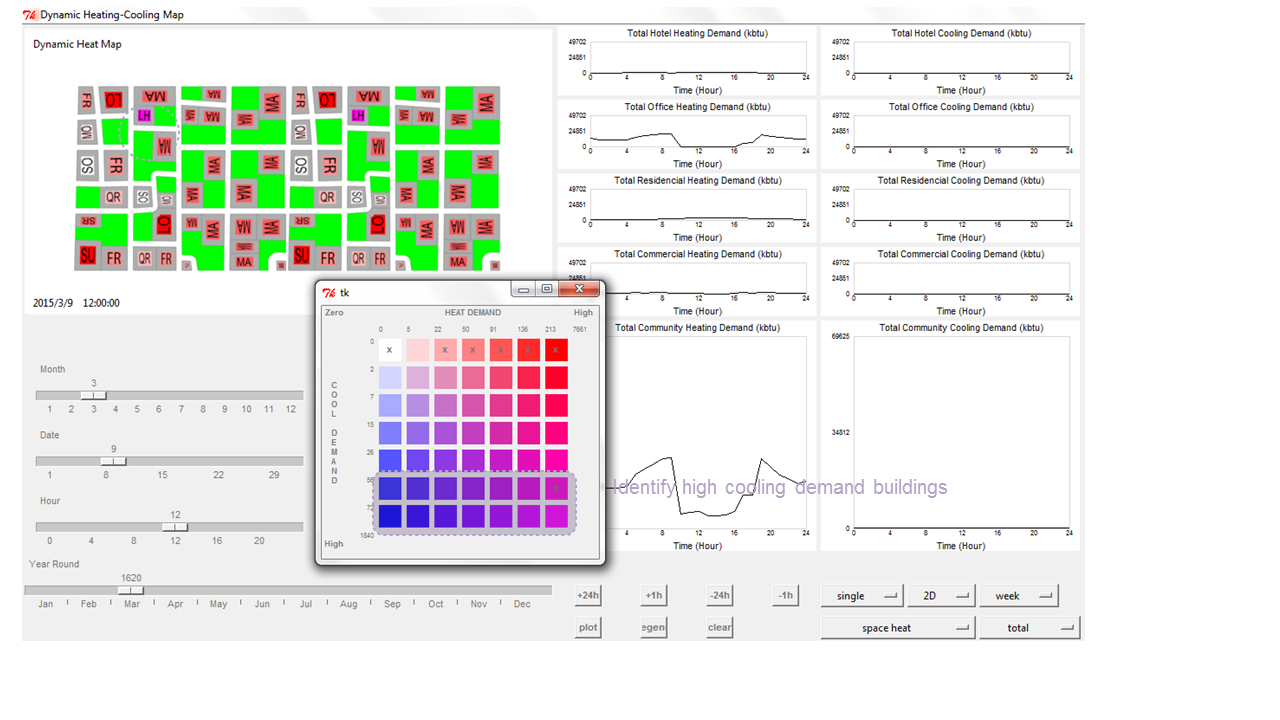
\includegraphics[width=0.7\linewidth]{highCooling.png}
  \caption[Identify Buildings with High Cooling Demand]{In the
    demonstration, buildings with a high cooling demand have colors on
    the bottom rows of the legend, thus Large Hotel and Large Office
    are identified as potential reject heat energy suppliers}
  \label{fig:highCooling}
\end{figure}

Users can then calculate the ``energy recovery potential'' in the
dynamic energy map with a specified time duration and step
(\fref{fig:ERP}).

\begin{figure}[h!]
  \centering
  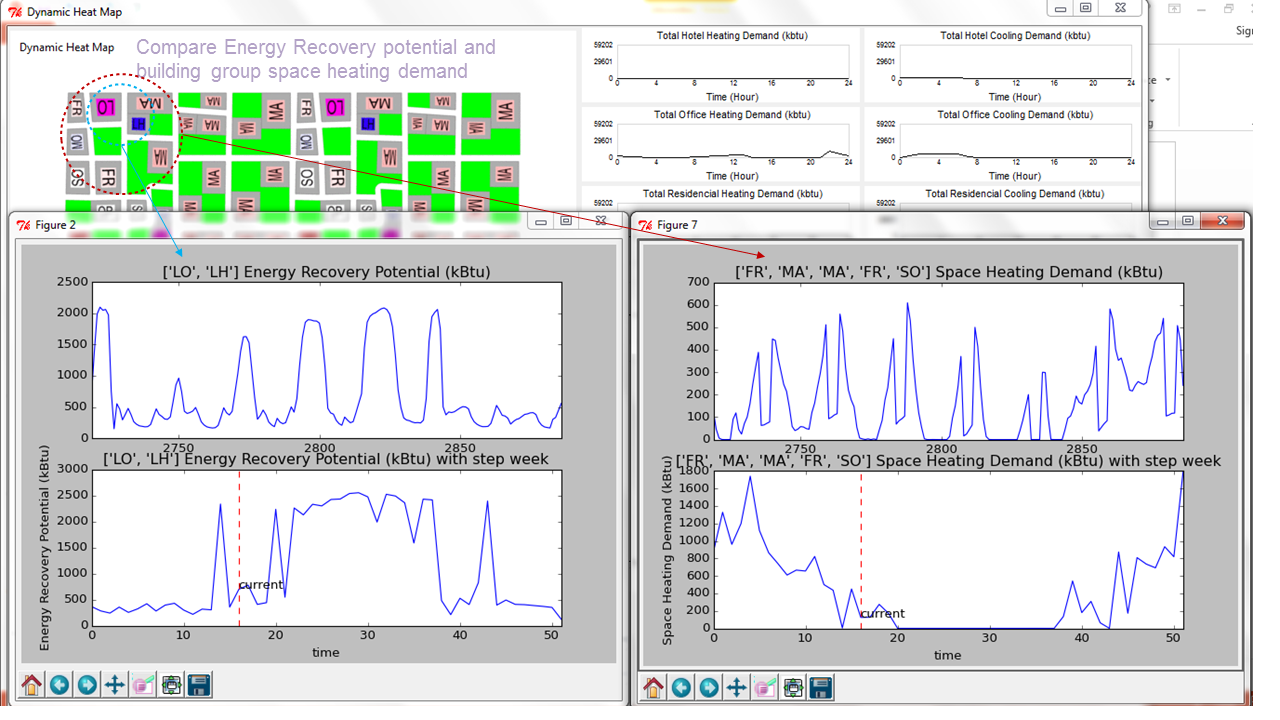
\includegraphics[width=0.7\linewidth]{ERP.png}
  \caption[Calculate Energy Recovery Potential]{The users can
    calculate the energy recovery potential of the group of reject
    heat suppliers (Large Office and Large Hotel). They can also
    calculate the total heat demand of the surrounding buildings with
    space heating demand (two FirstService Resturant, two Midrise
    Apartment and one Small Office).}
  \label{fig:ERP}
\end{figure}

\subsection{Use Case II: Sizing CHP Plant}
Two variables are crucial in sizing a CHP plant: 1) the heating demand
including space heating and service hot water 2) electricity
demand. For the current dynamic energy map interface, a 2D/3D
choropleth map are presented in the main map display window with the
heating demand and electricity demand encoded with a seven-class
bivariate choropleth legend as in \fref{fig:legendCHP}.
\begin{figure}[h!]
  \centering
  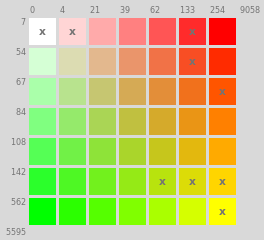
\includegraphics[width=0.3\linewidth]{legendCHP.png}
  \caption[Legend for Heat and Power Map]{Legend for Heat and Power
    Map}
  \label{fig:legendCHP}
\end{figure}
The dynamic plot on the right of the interface depicts the heating and
electricity demand of the four building sectors and the community
(\fref{fig:interfaceCHP}).
\begin{figure}[h!]
  \centering
  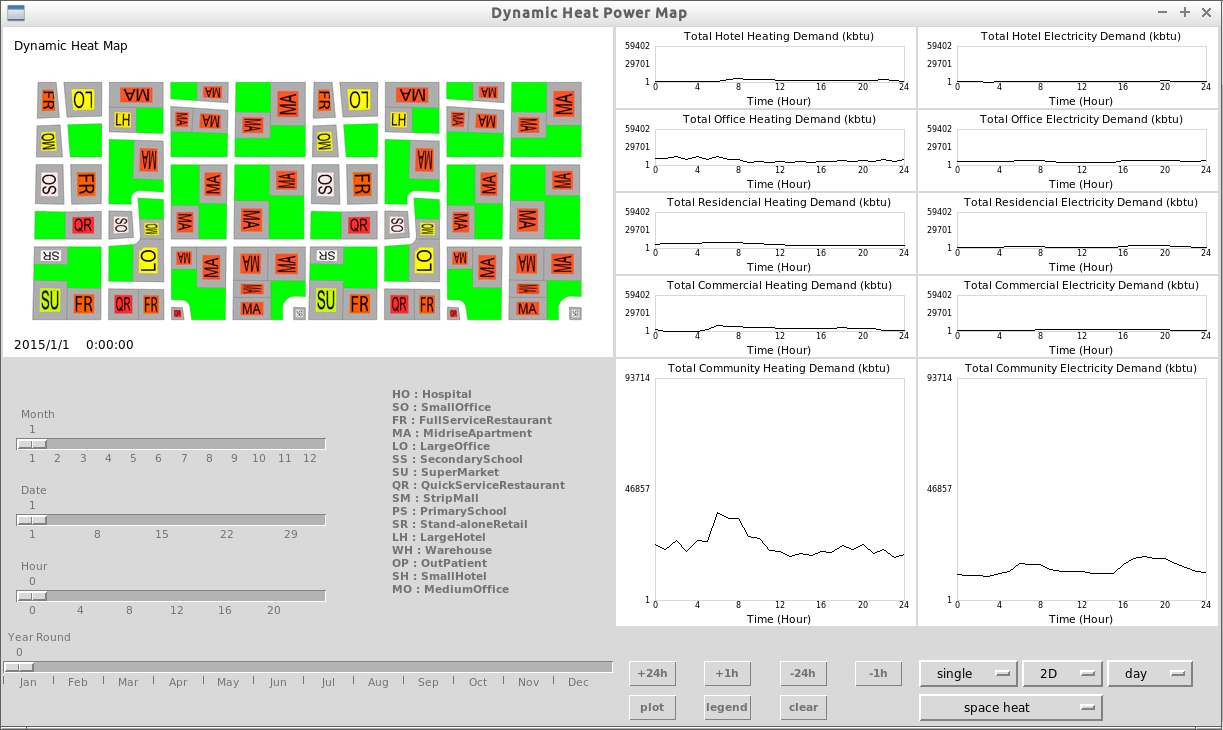
\includegraphics[width=0.7\linewidth]{interfaceCHP.png}
  \caption[Interface for CHP Sizing]{The interface displays the
    heating and electricity demand on the right}
  \label{fig:interfaceCHP}
\end{figure}

The user can inspect more detailed heating energy and power demand of
the community with the ``plot'' button with the ``community'' option
in the option menu selected.
\begin{figure}[h!]
  \centering
  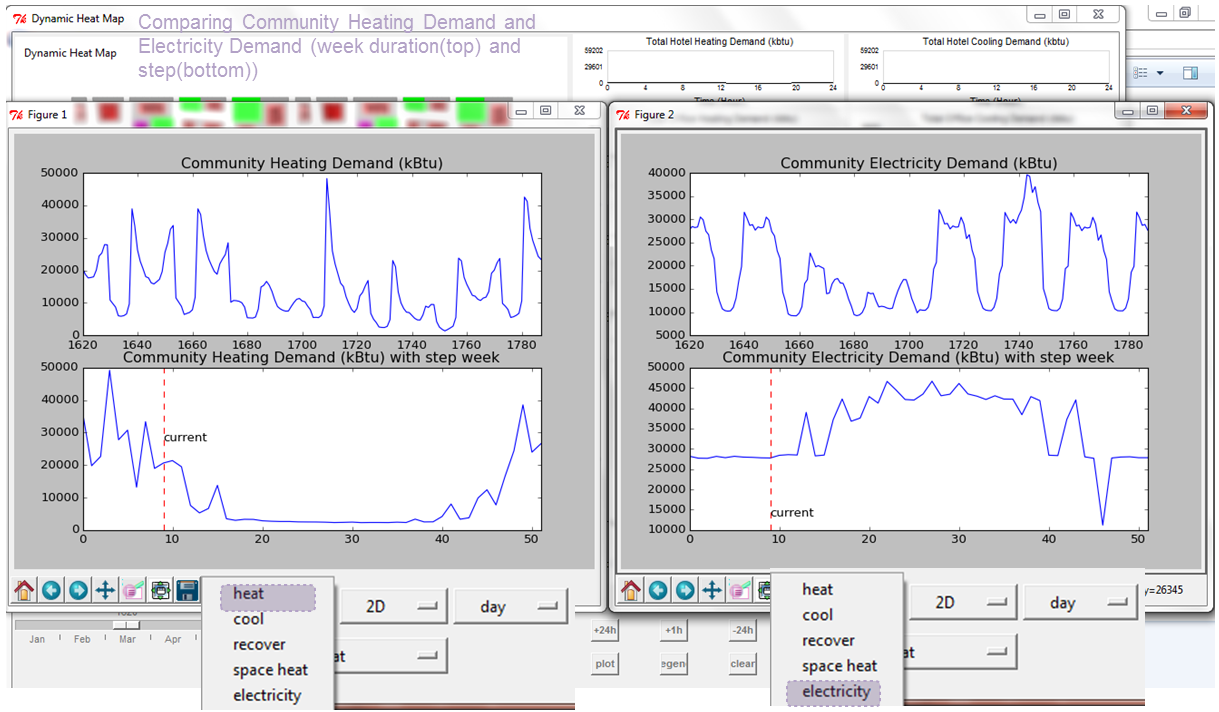
\includegraphics[width=0.7\linewidth]{heatPowerDemand.png}
  \caption[Comparing Community Heating and Electricity Demand]{In this
    example, the users compare the week-wise heating and electricity
    demand}
  \label{fig:heatPowerDemand}
\end{figure}

\section {Implementation tools and strategy}
The software or platform involved in the project include EnergyPlus
for building simulation, CityEngine for 3D modeling and image
generation. 

Imagemagic is used for converting and resizing images. For the
creation of animated maps, ``ffmepeg'' was used for connect image
sequences to animation.

Python 2.7 for interface design. The interface is written
in Python2.7 with standard Tkinter graphic package including the data
plot section. Pandas and numpy packages are used in data
manipulation. Matplotlib and ggplot are used for creating data plots.

\begin{comment}
\section{Future Trends}
Harrower and Fabrikant mentioned that the chanllenge of using animated
maps is the overflow of information and the vulnerability to
distraction~\cite{Harrower2008}. One example mentioned by Harrower and
Fabrikant is the comparison of color on the map and that on the legend
becomes difficult for animated maps as a result of the changing of
images. They proposed the audio legend approach of strengthening
information convey with minimized
distraction~\cite{Harrower2008}. This might become one of the next
extensions of the current Dynamic Energy Map interface design.

They also suggested that the difference in time should have different
visual representations in data display~\cite{Harrower2008}. Peuquet
claimed that ``The development of temporal analytical capabilities in
GIS such as temporal queries requires basic topological structures in
both time and space''~\cite{Peuquet1994}. Thus the different spatial
representation seems to be a natural choice for adapting to different
temporal resolution and scale.



The non-interactive animation could be found
\href{http://www.armechxyj.com/energy-mapping.html#redblueAnime3d}{through
  this link}.
\end{comment}